\begin{figure}[H]
    \centering
    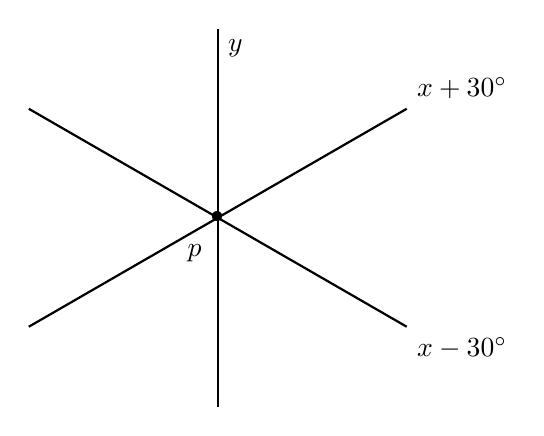
\begin{tikzpicture}[thick, scale=0.8]
        \draw (0, -3) -- (0, 3) node[anchor=north west] {$y$};
        \draw (-3, 1.7302) -- (3, -1.7302)
        node[anchor=north west] {$x - 30^\circ$};
        \draw (-3, -1.7302) -- (3, 1.7302)
        node[anchor=south west] {$x + 30^\circ$};
        \node[label=250:$p$] (p) at (0, 0) {\textbullet};
    \end{tikzpicture}
    \caption[Exemplo de cones do algoritmo estático]{A reta paralela
    ao eixo $y$ que passa por $p$ e as retas $x \pm 30^\circ$.}
    \label{fig:parestatico:cones}
\end{figure}